\documentclass[a4paper]{book}
\usepackage{makeidx}
\usepackage{natbib}
\usepackage{graphicx}
\usepackage{multicol}
\usepackage{float}
\usepackage{listings}
\usepackage{color}
\usepackage{ifthen}
\usepackage[table]{xcolor}
\usepackage{textcomp}
\usepackage{alltt}
\usepackage{ifpdf}
\ifpdf
\usepackage[pdftex,
            pagebackref=true,
            colorlinks=true,
            linkcolor=blue,
            unicode
           ]{hyperref}
\else
\usepackage[ps2pdf,
            pagebackref=true,
            colorlinks=true,
            linkcolor=blue,
            unicode
           ]{hyperref}
\usepackage{pspicture}
\fi
\usepackage[utf8]{inputenc}
\usepackage{polski}
\usepackage[T1]{fontenc}

\usepackage{mathptmx}
\usepackage[scaled=.90]{helvet}
\usepackage{courier}
\usepackage{sectsty}
\usepackage[titles]{tocloft}
\usepackage{doxygen}
\lstset{language=C++,inputencoding=utf8,basicstyle=\footnotesize,breaklines=true,breakatwhitespace=true,tabsize=8,numbers=left }
\makeindex
\setcounter{tocdepth}{3}
\renewcommand{\footrulewidth}{0.4pt}
\renewcommand{\familydefault}{\sfdefault}
\hfuzz=15pt
\setlength{\emergencystretch}{15pt}
\hbadness=750
\tolerance=750
\begin{document}
\hypersetup{pageanchor=false,citecolor=blue}
\begin{titlepage}
\vspace*{7cm}
\begin{center}
{\Large \-P\-A\-M\-S\-I -\/ \-Piotr \-Wilkosz \\[1ex]\large 1 }\\
\vspace*{1cm}
{\large \-Wygenerowano przez Doxygen 1.7.6.1}\\
\vspace*{0.5cm}
{\small Sun Mar 2 2014 16:19:52}\\
\end{center}
\end{titlepage}
\clearemptydoublepage
\pagenumbering{roman}
\tableofcontents
\clearemptydoublepage
\pagenumbering{arabic}
\hypersetup{pageanchor=true,citecolor=blue}
\chapter{\-Indeks klas}
\section{\-Hierarchia klas}
\-Ta lista dziedziczenia posortowana jest z grubsza, choć nie całkowicie, alfabetycznie\-:\begin{DoxyCompactList}
\item \contentsline{section}{algorytm}{\pageref{classalgorytm}}{}
\begin{DoxyCompactList}
\item \contentsline{section}{h\-\_\-sort}{\pageref{classh__sort}}{}
\item \contentsline{section}{kolejka\-\_\-lista}{\pageref{classkolejka__lista}}{}
\item \contentsline{section}{kolejka\-\_\-tablica}{\pageref{classkolejka__tablica}}{}
\item \contentsline{section}{m\-\_\-sort}{\pageref{classm__sort}}{}
\item \contentsline{section}{mnozenie}{\pageref{classmnozenie}}{}
\item \contentsline{section}{q\-\_\-sort}{\pageref{classq__sort}}{}
\item \contentsline{section}{stos\-\_\-lista}{\pageref{classstos__lista}}{}
\item \contentsline{section}{stos\-\_\-tablica}{\pageref{classstos__tablica}}{}
\end{DoxyCompactList}
\item \contentsline{section}{operacje}{\pageref{classoperacje}}{}
\item \contentsline{section}{queue\-\_\-array$<$ \-T\-Y\-P $>$}{\pageref{classqueue__array}}{}
\item \contentsline{section}{queue\-\_\-list$<$ \-T\-Y\-P $>$}{\pageref{classqueue__list}}{}
\item \contentsline{section}{stack\-\_\-array$<$ \-T\-Y\-P $>$}{\pageref{classstack__array}}{}
\item \contentsline{section}{stack\-\_\-list$<$ \-T\-Y\-P $>$}{\pageref{classstack__list}}{}
\end{DoxyCompactList}

\chapter{\-Indeks klas}
\section{\-Lista klas}
\-Tutaj znajdują się klasy, struktury, unie i interfejsy wraz z ich krótkimi opisami\-:\begin{DoxyCompactList}
\item\contentsline{section}{\hyperlink{classalgorytm}{algorytm} \\*\-Definicja klasy algorytm \-Jest to klasa bazowa, ktora ma za zadanie wczytac, przetworzyc i porownac dane z plikiem wzorcowym }{\pageref{classalgorytm}}{}
\item\contentsline{section}{\hyperlink{classmnozenie}{mnozenie} \\*\-Modeluje algorytm dokonujacy mnozenia kazdego elementu pliku wejsciowego przez 2 }{\pageref{classmnozenie}}{}
\item\contentsline{section}{\hyperlink{classoperacje}{operacje} \\*\-Klasa modeluje tablice z danymi i metody sluzace do operacji na niej }{\pageref{classoperacje}}{}
\end{DoxyCompactList}

\chapter{\-Indeks plików}
\section{Lista plików}
Tutaj znajduje się lista wszystkich plików z ich krótkimi opisami\-:\begin{DoxyCompactList}
\item\contentsline{section}{\hyperlink{algorytm_8cpp}{algorytm.\-cpp} \\*Plik zawiera definicje metod klas zdefiniowanych w pliku \hyperlink{algorytm_8hh}{algorytm.\-hh} }{\pageref{algorytm_8cpp}}{}
\item\contentsline{section}{\hyperlink{algorytm_8hh}{algorytm.\-hh} \\*Definicja klas wykonujacych operacje na zestawie danych wejsciowych }{\pageref{algorytm_8hh}}{}
\item\contentsline{section}{\hyperlink{drzewo_8hh}{drzewo.\-hh} }{\pageref{drzewo_8hh}}{}
\item\contentsline{section}{\hyperlink{graf_8cpp}{graf.\-cpp} }{\pageref{graf_8cpp}}{}
\item\contentsline{section}{\hyperlink{graf_8hh}{graf.\-hh} }{\pageref{graf_8hh}}{}
\item\contentsline{section}{\hyperlink{hashtab_8hh}{hashtab.\-hh} }{\pageref{hashtab_8hh}}{}
\item\contentsline{section}{\hyperlink{kolejka_8hh}{kolejka.\-hh} \\*Plik zawiera definicje klasy Kolejka Zaimplementowanej na 2 sposoby }{\pageref{kolejka_8hh}}{}
\item\contentsline{section}{\hyperlink{main_8cpp}{main.\-cpp} \\*Plik glowny }{\pageref{main_8cpp}}{}
\item\contentsline{section}{\hyperlink{operacje_8cpp}{operacje.\-cpp} }{\pageref{operacje_8cpp}}{}
\item\contentsline{section}{\hyperlink{operacje_8hh}{operacje.\-hh} }{\pageref{operacje_8hh}}{}
\item\contentsline{section}{\hyperlink{simplex_8cpp}{simplex.\-cpp} }{\pageref{simplex_8cpp}}{}
\item\contentsline{section}{\hyperlink{simplex_8hh}{simplex.\-hh} }{\pageref{simplex_8hh}}{}
\item\contentsline{section}{\hyperlink{statystyki_8cpp}{statystyki.\-cpp} }{\pageref{statystyki_8cpp}}{}
\item\contentsline{section}{\hyperlink{statystyki_8hh}{statystyki.\-hh} \\*Plik zawiera dekalracje funkcji odpowiedzialnych za przeprowadznaie statystyk }{\pageref{statystyki_8hh}}{}
\item\contentsline{section}{\hyperlink{stos_8hh}{stos.\-hh} \\*Plik zawiera definicje klasy {\ttfamily Stos} Zaimplementowana na 2 sposoby }{\pageref{stos_8hh}}{}
\item\contentsline{section}{\hyperlink{str__operacje_8cpp}{str\-\_\-operacje.\-cpp} }{\pageref{str__operacje_8cpp}}{}
\item\contentsline{section}{\hyperlink{str__operacje_8hh}{str\-\_\-operacje.\-hh} }{\pageref{str__operacje_8hh}}{}
\item\contentsline{section}{\hyperlink{tablica__asocjacyjna_8hh}{tablica\-\_\-asocjacyjna.\-hh} }{\pageref{tablica__asocjacyjna_8hh}}{}
\end{DoxyCompactList}

\chapter{\-Dokumentacja klas}
\hypertarget{classalgorytm}{\section{\-Dokumentacja klasy algorytm}
\label{classalgorytm}\index{algorytm@{algorytm}}
}


\-Definicja klasy algorytm \-Jest to klasa bazowa, ktora ma za zadanie wczytac, przetworzyc i porownac plik z plikiem wzorcowym.  




{\ttfamily \#include $<$algorytm.\-hh$>$}



\-Diagram dziedziczenia dla algorytm
\nopagebreak
\begin{figure}[H]
\begin{center}
\leavevmode
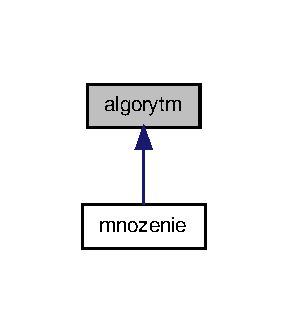
\includegraphics[width=138pt]{classalgorytm__inherit__graph}
\end{center}
\end{figure}
\subsection*{\-Metody publiczne}
\begin{DoxyCompactItemize}
\item 
\hyperlink{classalgorytm_a138ed27849535b192fec3d2e9f6a644f}{algorytm} (const char $\ast$plik1, const char $\ast$plik2)
\begin{DoxyCompactList}\small\item\em konstruktor kopiujacy -\/ przekazuje informacje o nazwach plikow, ktore zapisywane sa do pol klasy \end{DoxyCompactList}\item 
virtual void \hyperlink{classalgorytm_a85ba543fad39e8987bbda4ee698b5fec}{wykonaj} ()
\begin{DoxyCompactList}\small\item\em funkcja dokonuje operacji na pliku wejsciowym \end{DoxyCompactList}\item 
bool \hyperlink{classalgorytm_a167adca6239e12cb5d362fd7c905dde0}{porownaj} ()
\begin{DoxyCompactList}\small\item\em porownuje przetworzony plik z plikiem wzorcowym \end{DoxyCompactList}\item 
int \hyperlink{classalgorytm_acbd9260a0b2055acee485f737b960992}{ile\-\_\-danych} ()
\item 
vector$<$ float $>$ \hyperlink{classalgorytm_a244d9cbf20639faf0b60ae6cdae3c657}{jaki\-\_\-czas} ()
\end{DoxyCompactItemize}
\subsection*{\-Atrybuty publiczne}
\begin{DoxyCompactItemize}
\item 
vector$<$ float $>$ \hyperlink{classalgorytm_aac9e2179e0e956dbe0dc1239ebadb2e4}{czas}
\begin{DoxyCompactList}\small\item\em zawiera wyniki dzialania algorytmu \end{DoxyCompactList}\end{DoxyCompactItemize}
\subsection*{\-Atrybuty chronione}
\begin{DoxyCompactItemize}
\item 
int \hyperlink{classalgorytm_a2778c37f0ec06a30b7d494501c40e91a}{n}
\begin{DoxyCompactList}\small\item\em zawiera informacje o ilosci liczb w pliku \end{DoxyCompactList}\item 
const char $\ast$ \hyperlink{classalgorytm_ab911ca0437df967d0240651855e5a2a3}{plik\-We}
\begin{DoxyCompactList}\small\item\em zawiera nazwe pliku wejsciowego \end{DoxyCompactList}\item 
const char $\ast$ \hyperlink{classalgorytm_a19c2be15efb3e5e34bf177d50b746d93}{plik\-Wz}
\begin{DoxyCompactList}\small\item\em zawiera nazwe pliku wzorcowego \end{DoxyCompactList}\end{DoxyCompactItemize}


\subsection{\-Opis szczegółowy}
\-Definicja klasy algorytm \-Jest to klasa bazowa, ktora ma za zadanie wczytac, przetworzyc i porownac plik z plikiem wzorcowym. 

\-Definicja w linii 32 pliku algorytm.\-hh.



\subsection{\-Dokumentacja konstruktora i destruktora}
\hypertarget{classalgorytm_a138ed27849535b192fec3d2e9f6a644f}{\index{algorytm@{algorytm}!algorytm@{algorytm}}
\index{algorytm@{algorytm}!algorytm@{algorytm}}
\subsubsection[{algorytm}]{\setlength{\rightskip}{0pt plus 5cm}{\bf algorytm\-::algorytm} (
\begin{DoxyParamCaption}
\item[{const char $\ast$}]{plik1, }
\item[{const char $\ast$}]{plik2}
\end{DoxyParamCaption}
)\hspace{0.3cm}{\ttfamily  \mbox{[}inline\mbox{]}}}}\label{classalgorytm_a138ed27849535b192fec3d2e9f6a644f}


konstruktor kopiujacy -\/ przekazuje informacje o nazwach plikow, ktore zapisywane sa do pol klasy 


\begin{DoxyParams}{\-Parametry}
{\em plik1} & -\/ plik wejsciowy \\
\hline
{\em plik2} & -\/ plik wzorcowy \\
\hline
\end{DoxyParams}


\-Definicja w linii 56 pliku algorytm.\-hh.



\subsection{\-Dokumentacja funkcji składowych}
\hypertarget{classalgorytm_acbd9260a0b2055acee485f737b960992}{\index{algorytm@{algorytm}!ile\-\_\-danych@{ile\-\_\-danych}}
\index{ile\-\_\-danych@{ile\-\_\-danych}!algorytm@{algorytm}}
\subsubsection[{ile\-\_\-danych}]{\setlength{\rightskip}{0pt plus 5cm}int {\bf algorytm\-::ile\-\_\-danych} (
\begin{DoxyParamCaption}
{}
\end{DoxyParamCaption}
)}}\label{classalgorytm_acbd9260a0b2055acee485f737b960992}
\begin{DoxyReturn}{\-Zwraca}
ilosc liczb wejsciowych 
\end{DoxyReturn}


\-Definicja w linii 16 pliku algorytm.\-cpp.

\hypertarget{classalgorytm_a244d9cbf20639faf0b60ae6cdae3c657}{\index{algorytm@{algorytm}!jaki\-\_\-czas@{jaki\-\_\-czas}}
\index{jaki\-\_\-czas@{jaki\-\_\-czas}!algorytm@{algorytm}}
\subsubsection[{jaki\-\_\-czas}]{\setlength{\rightskip}{0pt plus 5cm}vector$<$ float $>$ {\bf algorytm\-::jaki\-\_\-czas} (
\begin{DoxyParamCaption}
{}
\end{DoxyParamCaption}
)}}\label{classalgorytm_a244d9cbf20639faf0b60ae6cdae3c657}


\-Definicja w linii 19 pliku algorytm.\-cpp.

\hypertarget{classalgorytm_a167adca6239e12cb5d362fd7c905dde0}{\index{algorytm@{algorytm}!porownaj@{porownaj}}
\index{porownaj@{porownaj}!algorytm@{algorytm}}
\subsubsection[{porownaj}]{\setlength{\rightskip}{0pt plus 5cm}bool {\bf algorytm\-::porownaj} (
\begin{DoxyParamCaption}
{}
\end{DoxyParamCaption}
)}}\label{classalgorytm_a167adca6239e12cb5d362fd7c905dde0}


porownuje przetworzony plik z plikiem wzorcowym 

\begin{DoxyReturn}{\-Zwraca}
true -\/ gdy pliki zgodne false -\/ w przeciwnym przypadku 
\end{DoxyReturn}


\-Definicja w linii 23 pliku algorytm.\-cpp.



\-Oto graf wywoływań tej funkcji\-:
\nopagebreak
\begin{figure}[H]
\begin{center}
\leavevmode
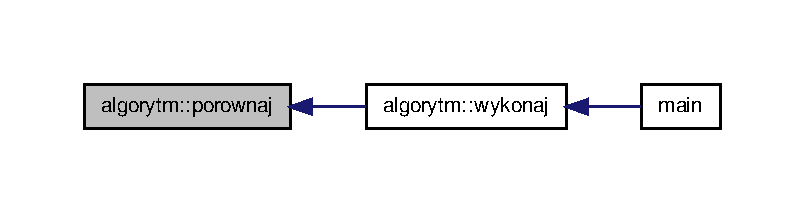
\includegraphics[width=350pt]{classalgorytm_a167adca6239e12cb5d362fd7c905dde0_icgraph}
\end{center}
\end{figure}


\hypertarget{classalgorytm_a85ba543fad39e8987bbda4ee698b5fec}{\index{algorytm@{algorytm}!wykonaj@{wykonaj}}
\index{wykonaj@{wykonaj}!algorytm@{algorytm}}
\subsubsection[{wykonaj}]{\setlength{\rightskip}{0pt plus 5cm}void {\bf algorytm\-::wykonaj} (
\begin{DoxyParamCaption}
{}
\end{DoxyParamCaption}
)\hspace{0.3cm}{\ttfamily  \mbox{[}virtual\mbox{]}}}}\label{classalgorytm_a85ba543fad39e8987bbda4ee698b5fec}


funkcja dokonuje operacji na pliku wejsciowym 



\-Reimplementowana w \hyperlink{classmnozenie_a2c5dc64610bb16af0ef18d142d6af2c0}{mnozenie}.



\-Definicja w linii 7 pliku algorytm.\-cpp.



\subsection{\-Dokumentacja atrybutów składowych}
\hypertarget{classalgorytm_aac9e2179e0e956dbe0dc1239ebadb2e4}{\index{algorytm@{algorytm}!czas@{czas}}
\index{czas@{czas}!algorytm@{algorytm}}
\subsubsection[{czas}]{\setlength{\rightskip}{0pt plus 5cm}vector$<$float$>$ {\bf algorytm\-::czas}}}\label{classalgorytm_aac9e2179e0e956dbe0dc1239ebadb2e4}


zawiera wyniki dzialania algorytmu 



\-Definicja w linii 50 pliku algorytm.\-hh.

\hypertarget{classalgorytm_a2778c37f0ec06a30b7d494501c40e91a}{\index{algorytm@{algorytm}!n@{n}}
\index{n@{n}!algorytm@{algorytm}}
\subsubsection[{n}]{\setlength{\rightskip}{0pt plus 5cm}int {\bf algorytm\-::n}\hspace{0.3cm}{\ttfamily  \mbox{[}protected\mbox{]}}}}\label{classalgorytm_a2778c37f0ec06a30b7d494501c40e91a}


zawiera informacje o ilosci liczb w pliku 



\-Definicja w linii 37 pliku algorytm.\-hh.

\hypertarget{classalgorytm_ab911ca0437df967d0240651855e5a2a3}{\index{algorytm@{algorytm}!plik\-We@{plik\-We}}
\index{plik\-We@{plik\-We}!algorytm@{algorytm}}
\subsubsection[{plik\-We}]{\setlength{\rightskip}{0pt plus 5cm}const char$\ast$ {\bf algorytm\-::plik\-We}\hspace{0.3cm}{\ttfamily  \mbox{[}protected\mbox{]}}}}\label{classalgorytm_ab911ca0437df967d0240651855e5a2a3}


zawiera nazwe pliku wejsciowego 



\-Definicja w linii 41 pliku algorytm.\-hh.

\hypertarget{classalgorytm_a19c2be15efb3e5e34bf177d50b746d93}{\index{algorytm@{algorytm}!plik\-Wz@{plik\-Wz}}
\index{plik\-Wz@{plik\-Wz}!algorytm@{algorytm}}
\subsubsection[{plik\-Wz}]{\setlength{\rightskip}{0pt plus 5cm}const char$\ast$ {\bf algorytm\-::plik\-Wz}\hspace{0.3cm}{\ttfamily  \mbox{[}protected\mbox{]}}}}\label{classalgorytm_a19c2be15efb3e5e34bf177d50b746d93}


zawiera nazwe pliku wzorcowego 



\-Definicja w linii 45 pliku algorytm.\-hh.



\-Dokumentacja dla tej klasy została wygenerowana z plików\-:\begin{DoxyCompactItemize}
\item 
\hyperlink{algorytm_8hh}{algorytm.\-hh}\item 
\hyperlink{algorytm_8cpp}{algorytm.\-cpp}\end{DoxyCompactItemize}

\hypertarget{classmnozenie}{\section{\-Dokumentacja klasy mnozenie}
\label{classmnozenie}\index{mnozenie@{mnozenie}}
}


modeluje algorytm dokonujacy mnozenia kazdego elementu pliku wejsciowego przez 2  




{\ttfamily \#include $<$algorytm.\-hh$>$}



\-Diagram dziedziczenia dla mnozenie\nopagebreak
\begin{figure}[H]
\begin{center}
\leavevmode
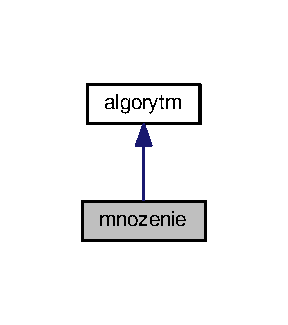
\includegraphics[width=138pt]{classmnozenie__inherit__graph}
\end{center}
\end{figure}


\-Diagram współpracy dla mnozenie\-:\nopagebreak
\begin{figure}[H]
\begin{center}
\leavevmode
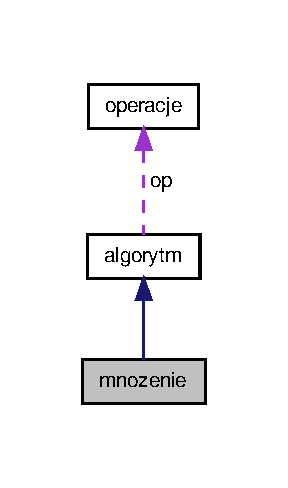
\includegraphics[width=138pt]{classmnozenie__coll__graph}
\end{center}
\end{figure}
\subsection*{\-Metody publiczne}
\begin{DoxyCompactItemize}
\item 
\hyperlink{classmnozenie_a105c483d60c621dc5c1855a04e285e3c}{mnozenie} (ifstream \&plik1, ifstream \&plik2, int \-N, int \-M)
\item 
void \hyperlink{classmnozenie_a5c97c36f9463bdf4eb7e34976a029930}{przelicz} ()
\begin{DoxyCompactList}\small\item\em wykonuje zalozony algorytm mnozenia elementow tablicy przez 2 \end{DoxyCompactList}\end{DoxyCompactItemize}


\subsection{\-Opis szczegółowy}
modeluje algorytm dokonujacy mnozenia kazdego elementu pliku wejsciowego przez 2 

\-Definicja w linii 125 pliku algorytm.\-hh.



\subsection{\-Dokumentacja konstruktora i destruktora}
\hypertarget{classmnozenie_a105c483d60c621dc5c1855a04e285e3c}{\index{mnozenie@{mnozenie}!mnozenie@{mnozenie}}
\index{mnozenie@{mnozenie}!mnozenie@{mnozenie}}
\subsubsection[{mnozenie}]{\setlength{\rightskip}{0pt plus 5cm}{\bf mnozenie\-::mnozenie} (
\begin{DoxyParamCaption}
\item[{ifstream \&}]{plik1, }
\item[{ifstream \&}]{plik2, }
\item[{int}]{\-N, }
\item[{int}]{\-M}
\end{DoxyParamCaption}
)\hspace{0.3cm}{\ttfamily  \mbox{[}inline\mbox{]}}}}\label{classmnozenie_a105c483d60c621dc5c1855a04e285e3c}
/brief konstruktor przekazuje do pol klasy informacje o nazwach pliku wejsciowego i wzorcowego 
\begin{DoxyParams}[1]{\-Parametry}
\mbox{\tt in}  & {\em plik1} & -\/ plik wejsciowy \\
\hline
\mbox{\tt in}  & {\em plik2} & -\/ plik wzorcowy \\
\hline
\mbox{\tt in}  & {\em \-N} & -\/ ilosc danych wejsciowych \\
\hline
\mbox{\tt in}  & {\em \-M} & -\/ ilosc powtorzen \\
\hline
\end{DoxyParams}


\-Definicja w linii 134 pliku algorytm.\-hh.



\subsection{\-Dokumentacja funkcji składowych}
\hypertarget{classmnozenie_a5c97c36f9463bdf4eb7e34976a029930}{\index{mnozenie@{mnozenie}!przelicz@{przelicz}}
\index{przelicz@{przelicz}!mnozenie@{mnozenie}}
\subsubsection[{przelicz}]{\setlength{\rightskip}{0pt plus 5cm}void {\bf mnozenie\-::przelicz} (
\begin{DoxyParamCaption}
{}
\end{DoxyParamCaption}
)\hspace{0.3cm}{\ttfamily  \mbox{[}virtual\mbox{]}}}}\label{classmnozenie_a5c97c36f9463bdf4eb7e34976a029930}


wykonuje zalozony algorytm mnozenia elementow tablicy przez 2 



\-Reimplementowana z \hyperlink{classalgorytm_aeefdd677ca8b9475a15547dcf8dd461f}{algorytm}.



\-Definicja w linii 81 pliku algorytm.\-cpp.



\-Dokumentacja dla tej klasy została wygenerowana z plików\-:\begin{DoxyCompactItemize}
\item 
\hyperlink{algorytm_8hh}{algorytm.\-hh}\item 
\hyperlink{algorytm_8cpp}{algorytm.\-cpp}\end{DoxyCompactItemize}

\chapter{\-Dokumentacja plików}
\hypertarget{algorytm_8cpp}{\section{\-Dokumentacja pliku algorytm.\-cpp}
\label{algorytm_8cpp}\index{algorytm.\-cpp@{algorytm.\-cpp}}
}


plik zawiera definicje metod klas zdefiniowanych w pliku \hyperlink{algorytm_8hh}{algorytm.\-hh}  


{\ttfamily \#include \char`\"{}algorytm.\-hh\char`\"{}}\*
\-Wykres zależności załączania dla algorytm.\-cpp\-:
\nopagebreak
\begin{figure}[H]
\begin{center}
\leavevmode
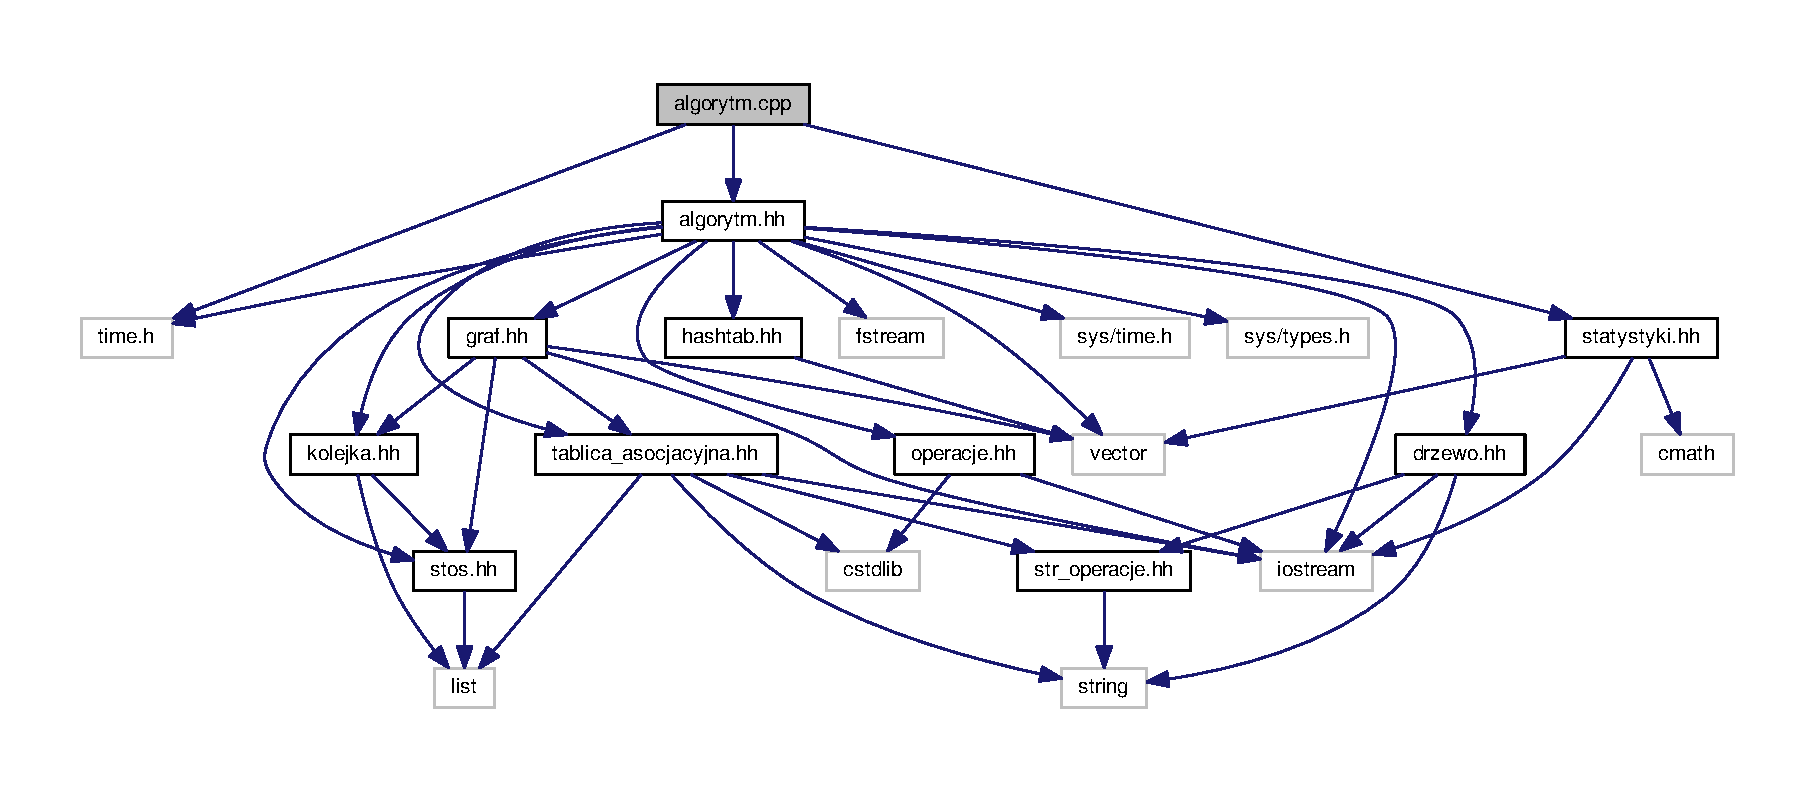
\includegraphics[width=350pt]{algorytm_8cpp__incl}
\end{center}
\end{figure}


\subsection{\-Opis szczegółowy}
plik zawiera definicje metod klas zdefiniowanych w pliku \hyperlink{algorytm_8hh}{algorytm.\-hh} 

\-Definicja w pliku \hyperlink{algorytm_8cpp_source}{algorytm.\-cpp}.


\hypertarget{algorytm_8hh}{\section{\-Dokumentacja pliku algorytm.\-hh}
\label{algorytm_8hh}\index{algorytm.\-hh@{algorytm.\-hh}}
}


\-Definicja klas wykonujacych operacje na zestawie danych wejsciowych.  


{\ttfamily \#include $<$iostream$>$}\*
{\ttfamily \#include $<$fstream$>$}\*
{\ttfamily \#include $<$vector$>$}\*
{\ttfamily \#include $<$ctime$>$}\*
{\ttfamily \#include $<$sys/time.\-h$>$}\*
{\ttfamily \#include $<$sys/types.\-h$>$}\*
\-Wykres zależności załączania dla algorytm.\-hh\-:
\nopagebreak
\begin{figure}[H]
\begin{center}
\leavevmode
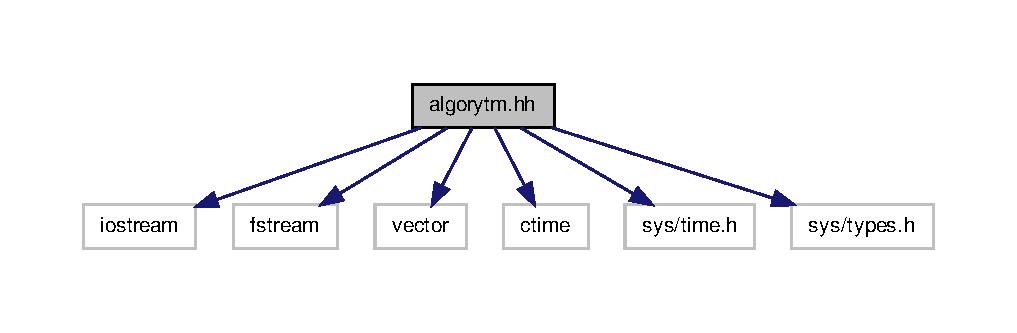
\includegraphics[width=350pt]{algorytm_8hh__incl}
\end{center}
\end{figure}
\-Ten wykres pokazuje, które pliki bezpośrednio lub pośrednio załączają ten plik\-:
\nopagebreak
\begin{figure}[H]
\begin{center}
\leavevmode
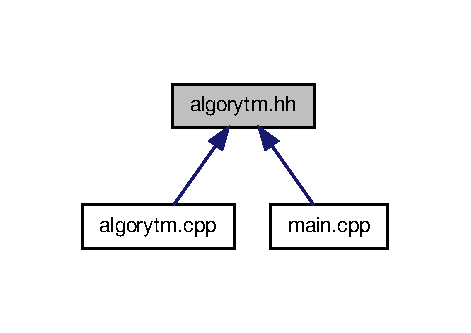
\includegraphics[width=226pt]{algorytm_8hh__dep__incl}
\end{center}
\end{figure}
\subsection*{\-Komponenty}
\begin{DoxyCompactItemize}
\item 
class \hyperlink{classalgorytm}{algorytm}
\begin{DoxyCompactList}\small\item\em \-Definicja klasy algorytm \-Jest to klasa bazowa, ktora ma za zadanie wczytac, przetworzyc i porownac plik z plikiem wzorcowym. \end{DoxyCompactList}\item 
class \hyperlink{classmnozenie}{mnozenie}
\begin{DoxyCompactList}\small\item\em modeluje algorytm dokonujacy mnozenia kazdego elementu pliku wejsciowego przez 2 \end{DoxyCompactList}\end{DoxyCompactItemize}


\subsection{\-Opis szczegółowy}
\-Definicja klas wykonujacych operacje na zestawie danych wejsciowych. 

\-Definicja w pliku \hyperlink{algorytm_8hh_source}{algorytm.\-hh}.


\hypertarget{main_8cpp}{\section{Dokumentacja pliku main.\-cpp}
\label{main_8cpp}\index{main.\-cpp@{main.\-cpp}}
}


plik glowny  


{\ttfamily \#include $<$iostream$>$}\\*
{\ttfamily \#include \char`\"{}algorytm.\-hh\char`\"{}}\\*
{\ttfamily \#include \char`\"{}statystyki.\-hh\char`\"{}}\\*
{\ttfamily \#include \char`\"{}operacje.\-hh\char`\"{}}\\*
{\ttfamily \#include \char`\"{}stos.\-hh\char`\"{}}\\*
{\ttfamily \#include \char`\"{}tablica\-\_\-asocjacyjna.\-hh\char`\"{}}\\*
{\ttfamily \#include \char`\"{}drzewo.\-hh\char`\"{}}\\*
{\ttfamily \#include \char`\"{}hashtab.\-hh\char`\"{}}\\*
{\ttfamily \#include \char`\"{}graf.\-hh\char`\"{}}\\*
{\ttfamily \#include $<$cstdlib$>$}\\*
{\ttfamily \#include $<$string$>$}\\*
Wykres zależności załączania dla main.\-cpp\-:\nopagebreak
\begin{figure}[H]
\begin{center}
\leavevmode
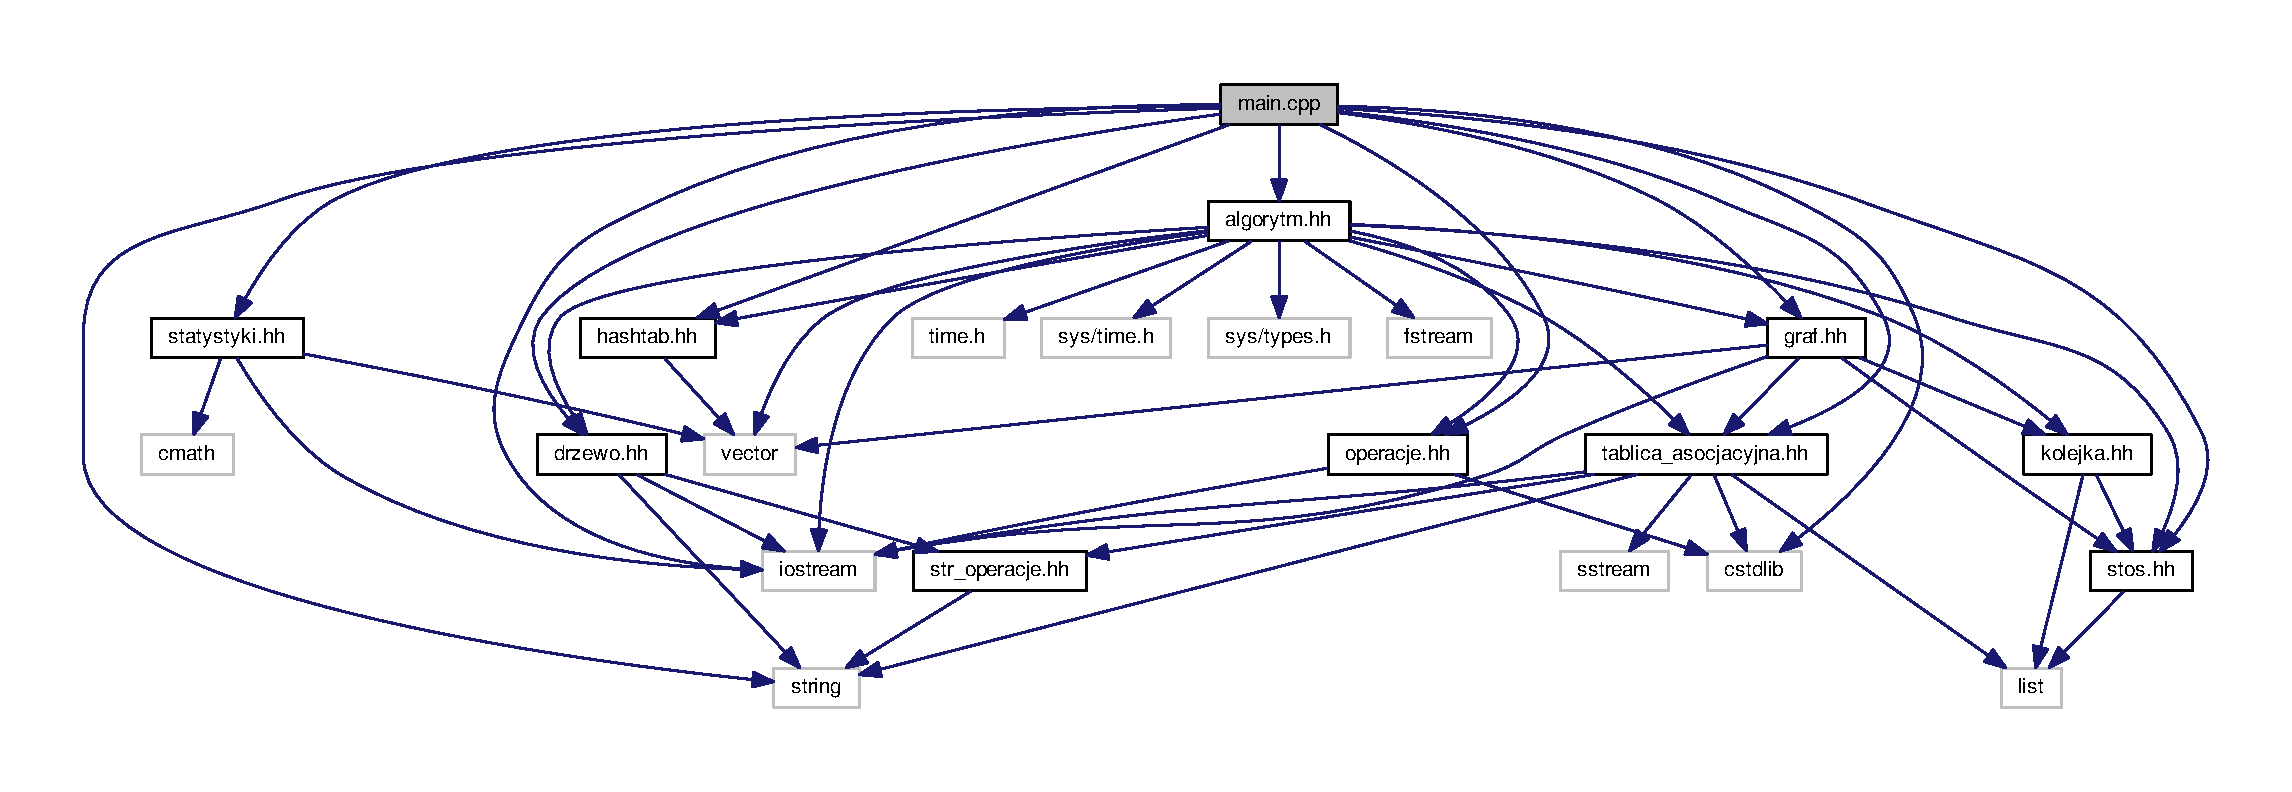
\includegraphics[width=350pt]{main_8cpp__incl}
\end{center}
\end{figure}
\subsection*{Funkcje}
\begin{DoxyCompactItemize}
\item 
int \hyperlink{main_8cpp_ae66f6b31b5ad750f1fe042a706a4e3d4}{main} ()
\end{DoxyCompactItemize}


\subsection{Opis szczegółowy}
plik glowny 

Definicja w pliku \hyperlink{main_8cpp_source}{main.\-cpp}.



\subsection{Dokumentacja funkcji}
\hypertarget{main_8cpp_ae66f6b31b5ad750f1fe042a706a4e3d4}{\index{main.\-cpp@{main.\-cpp}!main@{main}}
\index{main@{main}!main.cpp@{main.\-cpp}}
\subsubsection[{main}]{\setlength{\rightskip}{0pt plus 5cm}int main (
\begin{DoxyParamCaption}
{}
\end{DoxyParamCaption}
)}}\label{main_8cpp_ae66f6b31b5ad750f1fe042a706a4e3d4}


Definicja w linii 20 pliku main.\-cpp.



Oto graf wywołań dla tej funkcji\-:\nopagebreak
\begin{figure}[H]
\begin{center}
\leavevmode
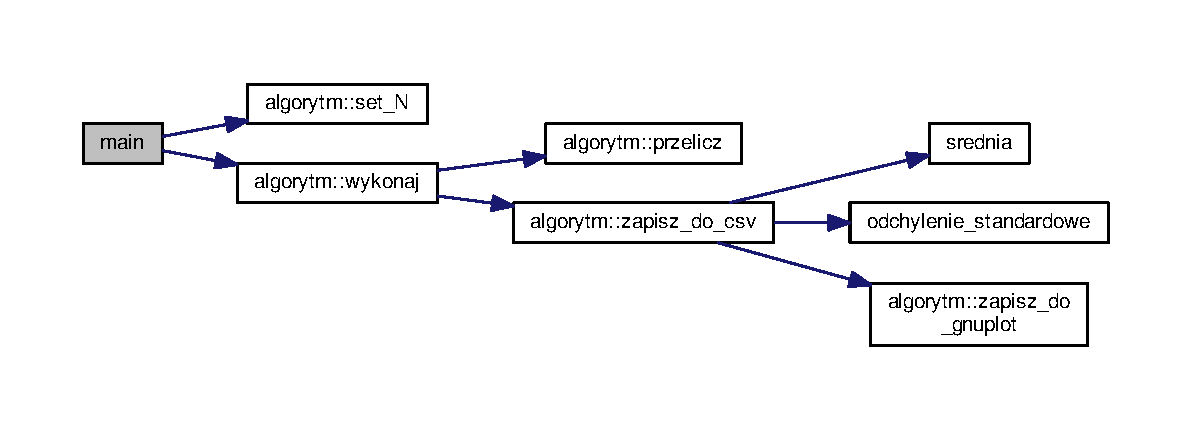
\includegraphics[width=350pt]{main_8cpp_ae66f6b31b5ad750f1fe042a706a4e3d4_cgraph}
\end{center}
\end{figure}



\hypertarget{statystyki_8cpp}{\section{\-Dokumentacja pliku statystyki.\-cpp}
\label{statystyki_8cpp}\index{statystyki.\-cpp@{statystyki.\-cpp}}
}
{\ttfamily \#include \char`\"{}statystyki.\-hh\char`\"{}}\*
\-Wykres zależności załączania dla statystyki.\-cpp\-:\nopagebreak
\begin{figure}[H]
\begin{center}
\leavevmode
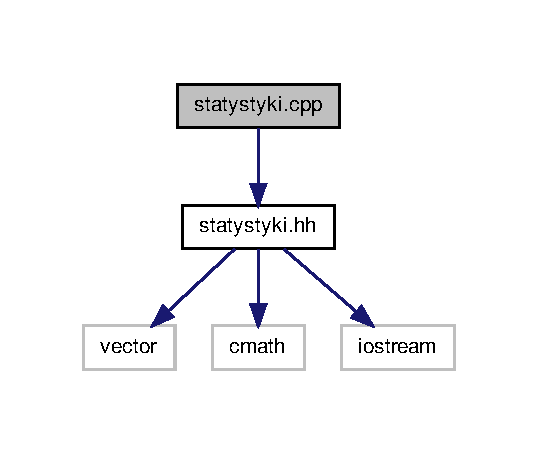
\includegraphics[width=258pt]{statystyki_8cpp__incl}
\end{center}
\end{figure}
\subsection*{\-Funkcje}
\begin{DoxyCompactItemize}
\item 
float \hyperlink{statystyki_8cpp_a978b972ebd4a834c47800d668ba8ecf2}{srednia} (float $\ast$tab, int rozmiar)
\begin{DoxyCompactList}\small\item\em funckja oblicza wartosc srednia \end{DoxyCompactList}\item 
float \hyperlink{statystyki_8cpp_a6648f32fbaacb03204231efea979cbf8}{odchylenie\-\_\-standardowe} (float \hyperlink{statystyki_8cpp_a978b972ebd4a834c47800d668ba8ecf2}{srednia}, float $\ast$tab, int rozmiar)
\begin{DoxyCompactList}\small\item\em funckja oblicza odchylenie standardowe \end{DoxyCompactList}\end{DoxyCompactItemize}


\subsection{\-Dokumentacja funkcji}
\hypertarget{statystyki_8cpp_a6648f32fbaacb03204231efea979cbf8}{\index{statystyki.\-cpp@{statystyki.\-cpp}!odchylenie\-\_\-standardowe@{odchylenie\-\_\-standardowe}}
\index{odchylenie\-\_\-standardowe@{odchylenie\-\_\-standardowe}!statystyki.cpp@{statystyki.\-cpp}}
\subsubsection[{odchylenie\-\_\-standardowe}]{\setlength{\rightskip}{0pt plus 5cm}float {\bf odchylenie\-\_\-standardowe} (
\begin{DoxyParamCaption}
\item[{float}]{srednia, }
\item[{float $\ast$}]{tab, }
\item[{int}]{rozmiar}
\end{DoxyParamCaption}
)}}\label{statystyki_8cpp_a6648f32fbaacb03204231efea979cbf8}


funckja oblicza odchylenie standardowe 


\begin{DoxyParams}{\-Parametry}
{\em tab} & -\/ kontener zawierajacy czasy wykonania algorytmu \\
\hline
{\em srednia} & -\/ wartosc srednia \\
\hline
{\em rozmiar} & -\/ rozmiar tablicy \\
\hline
\end{DoxyParams}
\begin{DoxyReturn}{\-Zwraca}
odchylenie standardowe 
\end{DoxyReturn}


\-Definicja w linii 16 pliku statystyki.\-cpp.



\-Oto graf wywoływań tej funkcji\-:\nopagebreak
\begin{figure}[H]
\begin{center}
\leavevmode
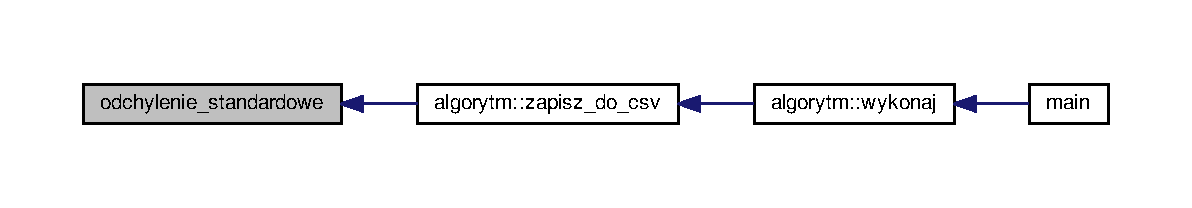
\includegraphics[width=350pt]{statystyki_8cpp_a6648f32fbaacb03204231efea979cbf8_icgraph}
\end{center}
\end{figure}


\hypertarget{statystyki_8cpp_a978b972ebd4a834c47800d668ba8ecf2}{\index{statystyki.\-cpp@{statystyki.\-cpp}!srednia@{srednia}}
\index{srednia@{srednia}!statystyki.cpp@{statystyki.\-cpp}}
\subsubsection[{srednia}]{\setlength{\rightskip}{0pt plus 5cm}float {\bf srednia} (
\begin{DoxyParamCaption}
\item[{float $\ast$}]{tab, }
\item[{int}]{rozmiar}
\end{DoxyParamCaption}
)}}\label{statystyki_8cpp_a978b972ebd4a834c47800d668ba8ecf2}


funckja oblicza wartosc srednia 


\begin{DoxyParams}{\-Parametry}
{\em tab} & -\/ kontener zawierajacy czasy wykonania algorytmu \\
\hline
{\em rozmiar} & -\/ rozmiar tablicy \\
\hline
\end{DoxyParams}
\begin{DoxyReturn}{\-Zwraca}
wartosc srednia 
\end{DoxyReturn}


\-Definicja w linii 3 pliku statystyki.\-cpp.



\-Oto graf wywoływań tej funkcji\-:\nopagebreak
\begin{figure}[H]
\begin{center}
\leavevmode
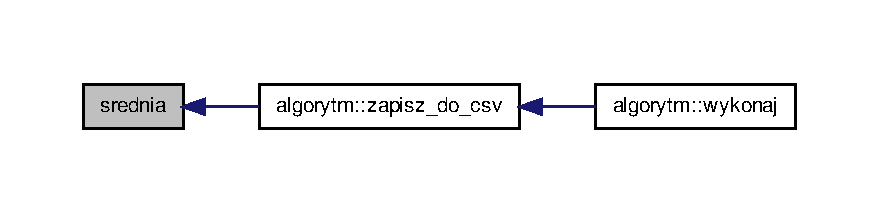
\includegraphics[width=350pt]{statystyki_8cpp_a978b972ebd4a834c47800d668ba8ecf2_icgraph}
\end{center}
\end{figure}



\hypertarget{statystyki_8hh}{\section{\-Dokumentacja pliku statystyki.\-hh}
\label{statystyki_8hh}\index{statystyki.\-hh@{statystyki.\-hh}}
}


plik zawiera dekalracje funkcji odpowiedzialnych za przeprowadznaie statystyk  


{\ttfamily \#include $<$vector$>$}\*
{\ttfamily \#include $<$cmath$>$}\*
{\ttfamily \#include $<$iostream$>$}\*
\-Wykres zależności załączania dla statystyki.\-hh\-:\nopagebreak
\begin{figure}[H]
\begin{center}
\leavevmode
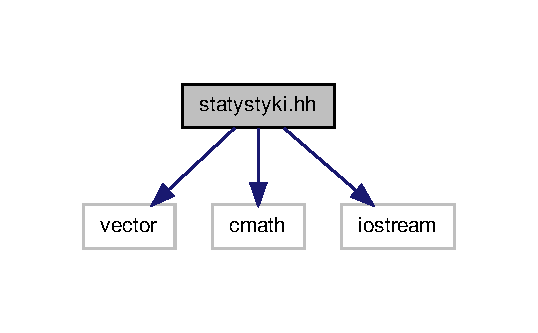
\includegraphics[width=258pt]{statystyki_8hh__incl}
\end{center}
\end{figure}
\-Ten wykres pokazuje, które pliki bezpośrednio lub pośrednio załączają ten plik\-:\nopagebreak
\begin{figure}[H]
\begin{center}
\leavevmode
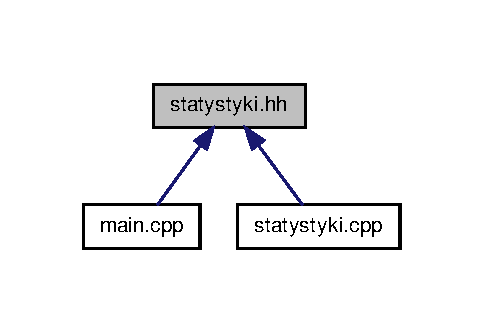
\includegraphics[width=322pt]{statystyki_8hh__dep__incl}
\end{center}
\end{figure}
\subsection*{\-Funkcje}
\begin{DoxyCompactItemize}
\item 
float \hyperlink{statystyki_8hh_a978b972ebd4a834c47800d668ba8ecf2}{srednia} (float $\ast$tab, int rozmiar)
\begin{DoxyCompactList}\small\item\em funckja oblicza wartosc srednia \end{DoxyCompactList}\item 
float \hyperlink{statystyki_8hh_a6648f32fbaacb03204231efea979cbf8}{odchylenie\-\_\-standardowe} (float \hyperlink{statystyki_8cpp_a978b972ebd4a834c47800d668ba8ecf2}{srednia}, float $\ast$tab, int rozmiar)
\begin{DoxyCompactList}\small\item\em funckja oblicza odchylenie standardowe \end{DoxyCompactList}\end{DoxyCompactItemize}


\subsection{\-Opis szczegółowy}
plik zawiera dekalracje funkcji odpowiedzialnych za przeprowadznaie statystyk 

\-Definicja w pliku \hyperlink{statystyki_8hh_source}{statystyki.\-hh}.



\subsection{\-Dokumentacja funkcji}
\hypertarget{statystyki_8hh_a6648f32fbaacb03204231efea979cbf8}{\index{statystyki.\-hh@{statystyki.\-hh}!odchylenie\-\_\-standardowe@{odchylenie\-\_\-standardowe}}
\index{odchylenie\-\_\-standardowe@{odchylenie\-\_\-standardowe}!statystyki.hh@{statystyki.\-hh}}
\subsubsection[{odchylenie\-\_\-standardowe}]{\setlength{\rightskip}{0pt plus 5cm}float {\bf odchylenie\-\_\-standardowe} (
\begin{DoxyParamCaption}
\item[{float}]{srednia, }
\item[{float $\ast$}]{tab, }
\item[{int}]{rozmiar}
\end{DoxyParamCaption}
)}}\label{statystyki_8hh_a6648f32fbaacb03204231efea979cbf8}


funckja oblicza odchylenie standardowe 


\begin{DoxyParams}{\-Parametry}
{\em tab} & -\/ kontener zawierajacy czasy wykonania algorytmu \\
\hline
{\em srednia} & -\/ wartosc srednia \\
\hline
{\em rozmiar} & -\/ rozmiar tablicy \\
\hline
\end{DoxyParams}
\begin{DoxyReturn}{\-Zwraca}
odchylenie standardowe 
\end{DoxyReturn}


\-Definicja w linii 16 pliku statystyki.\-cpp.



\-Oto graf wywoływań tej funkcji\-:\nopagebreak
\begin{figure}[H]
\begin{center}
\leavevmode
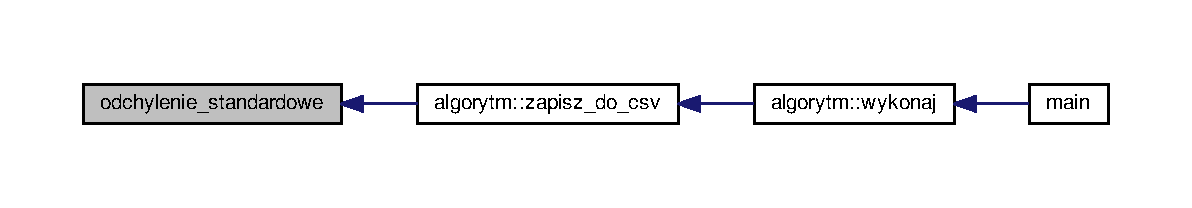
\includegraphics[width=350pt]{statystyki_8hh_a6648f32fbaacb03204231efea979cbf8_icgraph}
\end{center}
\end{figure}


\hypertarget{statystyki_8hh_a978b972ebd4a834c47800d668ba8ecf2}{\index{statystyki.\-hh@{statystyki.\-hh}!srednia@{srednia}}
\index{srednia@{srednia}!statystyki.hh@{statystyki.\-hh}}
\subsubsection[{srednia}]{\setlength{\rightskip}{0pt plus 5cm}float {\bf srednia} (
\begin{DoxyParamCaption}
\item[{float $\ast$}]{tab, }
\item[{int}]{rozmiar}
\end{DoxyParamCaption}
)}}\label{statystyki_8hh_a978b972ebd4a834c47800d668ba8ecf2}


funckja oblicza wartosc srednia 


\begin{DoxyParams}{\-Parametry}
{\em tab} & -\/ kontener zawierajacy czasy wykonania algorytmu \\
\hline
{\em rozmiar} & -\/ rozmiar tablicy \\
\hline
\end{DoxyParams}
\begin{DoxyReturn}{\-Zwraca}
wartosc srednia 
\end{DoxyReturn}


\-Definicja w linii 3 pliku statystyki.\-cpp.



\-Oto graf wywoływań tej funkcji\-:\nopagebreak
\begin{figure}[H]
\begin{center}
\leavevmode
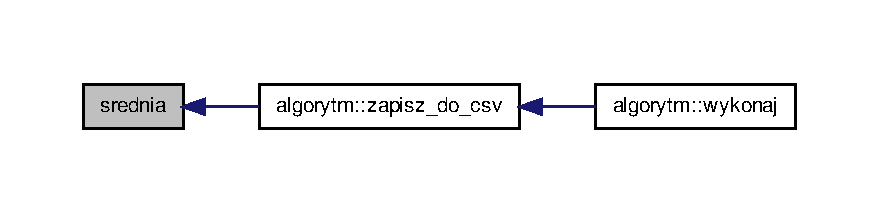
\includegraphics[width=350pt]{statystyki_8hh_a978b972ebd4a834c47800d668ba8ecf2_icgraph}
\end{center}
\end{figure}



\hypertarget{strona_8dox}{\section{\-Dokumentacja pliku strona.\-dox}
\label{strona_8dox}\index{strona.\-dox@{strona.\-dox}}
}

\printindex
\end{document}
